\section{Rancangan Solusi}
\label{sec:rancangan-solusi}

\subsection{Gambaran Umum}
Dengan segala kebutuhan yang sudah dianalisis, maka akan dibuat beberapa komponen penyusun sistem. Rencananya, sistem kontrol fleksibel akan dikembangkan dari luar kubernetes cluster sedangkan \textit{Elastic Search} itu sendiri diletakkan didalam kubernetes. Integrasi dengan API \textit{Elastic Search} akan melalui \textit{service} yang disediakan kubernetes sedangkan untuk mengontrol kubernetesnya sendiri akan digunakan \textit{Kubernetes Client Library}. Komponen penyusun dirancangkan diantaranya sebagai berikut.

\begin{enumerate}
    \item \textbf{Konfigurasi dan \textit{File Rule}}
    
    Konfigurasi dan \textit{File Rule} akan berinteraksi langsung dengan pengguna. Konfigurasi akan dibaca oleh mayoritas komponen sebagai pengaturan terhadap sistem sedangkan file rule yang di\textit{parse} oleh \textit{rule manager} untuk mengatur trigger dari \textit{resource controller} melakukan kontrol fleksibel terhadap alokasi sumber daya.

    \item \textbf{Kubernetes dan \textit{Elastic Search}}
    
    \textit{Elastic Search} akan diletakkan pada sebuah \textit{pods} di dalam sebuah \textit{cluster Kubernetes}. Dibuatkan sebuah \textit{service} agar \textit{Elastic Search} dapat diakses dari luar \textit{cluster}.
    
    \item \textbf{\textit{Predictor}}
    
    \textit{Predictor} akan berisikan model ARIMA untuk setiap variabel yang telah ditentukan. Model-model ini akan digunakan untuk memprediksi nilai variabel pada waktu selanjutnya sesuai permintaan \textit{rule manager}. Karena setiap rule mungkin untuk memiliki keperluan data untuk waktu prediksi yang berbeda.

    \item \textbf{\textit{Metrics Fetcher}}
    
    Komponen \textit{Metrics Fetcher} bertugas untuk menembak \href{https://www.elastic.co/guide/en/elasticsearch/reference/current/cluster-nodes-stats.html}{\textit{Node Stats API}} yang dimiliki oleh \textit{Elastic Search} dan meneruskannya kepada komponen \textit{Predictor} untuk melatih model.

    \item \textbf{\textit{Rule Manager}}
    
    Komponen \textit{Rule Manager} akan melakukan parsing terhadap file rule yang telah diisi oleh pengguna dan mengatur \textit{trigger}. Selain itu, komponen ini akan memberikan informasi tentang waktu prediksi yang diperlukan berdasarkan \textit{rule} yang telah dibuat oleh pengguna.

    \item \textbf{\textit{Resource Controller}}
    
    Komponen \textit{Resource Controller} akan memanfaatkan \textit{Kubernetes Client Library} untuk mengubah spesifikasi \textit{deployment} sehingga alokasi sumber daya dapat berubah. Pada pembuatan komponen ini, harus dilakukan eksperimen \textit{In-place Resource Resize} untuk mengubah alokasi sumber daya tanpa melakukan \textit{restart}.

    \item \textbf{\textit{Flexible Control}}
    
    Komponen \textit{Flexible Control} adalah komponen \textit{high-level} yang akan mengintegrasikan dan mengkolaborasikan komponen-komponen yang disebutkan sebelumnya.
\end{enumerate}

\subsection{Model Prediksi}

Model prediksi yang akan digunakan dalam solusi ini adalah ARIMA. Untuk perbandingan dan penjelasan dengan model-model lain dapat dilihat sebagai berikut.

\begin{enumerate}
    \item \textbf{ARIMA dengan LSTM dan Bi-LSTM}

    ARIMA adalah teknik model prediksi time series yang umum digunakan karena kemudahannya diinterpretasi dan dapat memperhitungkan pola data musiman atau tren yang simpleks. Namun, teknik ARIMA memerlukan banyak pengetahuan tentang data dan dapat memerlukan waktu yang lama untuk membangun model yang baik. Di satu sisi, LSTM yang memakai \textit{neural network} dapat memperhitungkan hubungan yang kompleks antara data historis dan bisa menangani data dengan dimensi yang tinggi. Teknik ini dapat memperhitungkan pola yang berubah dari waktu ke waktu. Kelemahan LSTM sendiri adalah pada kompleksitas perhitungan yang diperlukan untuk membangun model dan interpretasinya yang sulit dari hasil prediksi.

    Secara umum, ARIMA bisa menjadi pilihan yang baik untuk membangun model dengan data yang relatif sederhana dengan kekurangannya adalah waktu yang sangat lama untuk membangun sebuah model. Sedangkan, LSTM merupakah pilihan yang baik apabila data memiliki hubungan yang kompleks dan pola yang berubah dari waktu ke waktu dengan \textit{tradeoff} berupa dibutuhkan percobaan untuk melakukan konfigurasi model serta memikirkan algoritma dan berisiko untuk \textit{overfitting}.

    \item \textbf{ARIMA dengan SARIMA}
    
    Perbedaan dua model ini adalah ARIMA tidak dapat menangkap komponen musiman, sehingga tidak cocok untuk data yang memiliki fluktuasi musiman yang signifikan, seperti data yang bervariasi secara periodik. Di sisi lain, SARIMA adalah pengembangan dari ARIMA yang dapat menangani data dengan komponen musiman. SARIMA memperluas model ARIMA dengan tambahan komponen musiman untuk memodelkan fluktuasi periodik dalam data. Dengan demikian, SARIMA lebih cocok untuk memprediksi pola musiman, seperti data yang meningkat atau menurun secara periodik.

    Dalam hal ini, jika data dapat menunjukkan pola musiman yang jelas seperti faktor cuaca, hari libur, dan sebagainya, lebih tepat untuk menggunakan metode SARIMA. Namun, jika data tersebut cenderung tidak memiliki pola musiman yang kuat, maka metode ARIMA bisa menjadi pilihan yang lebih sederhana dan sesuai.

    \item \textbf{ARIMA dengan VARMAX}
    
    VARMAX adalah pengembangan dari metode VAR (\textit{Vector Autoregression}) yang digunakan untuk data time series multivariat, yang berarti melibatkan lebih dari satu variabel yang saling mempengaruhi. VARMAX memperluas kemampuan VAR dengan menambahkan komponen moving average sehingga dapat memodelkan hubungan yang lebih kompleks antara berbagai variabel. Sehingga, apabila data melibatkan banyak variabel yang saling mempengaruhi, maka VARMAX sangat cocok untuk dipakai karena VARMAX mempertimbangkan kompleksitas dan hubungan antar variabel.

\end{enumerate}

Oleh karena ini, pada tugas akhir ini pemakaian ARIMA didasari atas konsiderasi pada poin berikut.

\begin{enumerate}
    \item ARIMA lebih sederhana dibandingkan dengan LSTM dan Bi-LSTM.
    \item SARIMA membutuhkan pola musiman data yang jelas, yang tidak bisa dipastikan saat penulisan tugas akhir.
    \item Tidak ada keperluan untuk melibatkan hubungan antar variabel.
\end{enumerate}

\subsection{Sistem \textit{Rule}}

Dalam melakukan pemasangan \textit{autoscaler}, umumnya pengelola akan melakukan pengubahan \textit{treshold} dan jumlah \textit{request} serta \textit{limit} sumber daya untuk sebuah \textit{pods}. Apabila suatu saat terdapat perubahan pola penggunaan, maka pengelola harus menyesuaikan konfigurasi tersebut. Hal ini dapat dilakukan dengan cara memonitoring \textit{cluster} secara berkala dan melakukan perubahan konfigurasi secara manual. Namun, hal ini akan memakan waktu dan tenaga yang tidak sedikit. Oleh karena itu, dibutuhkan sebuah sistem yang dapat melakukan perubahan konfigurasi secara otomatis berdasarkan pola penggunaan yang terjadi. Secara umum, sistem \textit{rule} yang akan dibuat akan memiliki fungsional sebagai berikut.

\begin{enumerate}
    \item Terdapat beberapa kondisi yang dapat melakukan \textit{trigger} scaling.
    \item Terdapat sebuah konfigurasi aksi yang akan dilakukan apabila kondisi terpenuhi.
    \item Terdapat variabel \textit{user-defined} yang bisa digunakan oleh pengguna untuk perantara antar kondisi atau menggabungkan beberapa kondisi atau menjadi \textit{dynamic treshold} karena kondisi lain terpenuhi.
\end{enumerate}

\subsection{Arsitektur Sistem}
\label{sec:arsitektur-sistem}

Arsitektur sistem akan mengikuti \textbf{MAPE Loop} yang direferensikan dari riset terkait, \parencite{riset1}. Gambar arsitektur ini bisa dilihat pada gambar \ref{fig:mape}. Berikut adalah rancangan fase dengan arsitektur tersebut.

\begin{enumerate}
    \item \bfseries \textit{Monitor} \normalfont
    
        Fase ini akan menarik data dari \textit{Application Metric Collector}, yang pada konteks tugas akhir ini akan menarik dari \textit{Node Stats API} milik \textit{Elastic Search}.
    \item \bfseries \textit{Analyse} \normalfont
    
        Model prediksi akan memanfaatkan data yang didapat dari fase sebelumnya untuk melakukan analisa dan prediksi yang akan datang. Setelah berhasil memproses data tersebut, fase dilanjutkan ke fase \textit{Planning}.
    \item \bfseries \textit{Planning} \normalfont
    
        Fase ini akan melakukan pengecekan semua kondisi yang telah dikonfigurasi oleh pengelola. Pertama-tama, sistem akan melihat semua kebutuhan variabel prediksi. Lalu melakukan prediksi dengan menggunakan model prediksi yang sudah dibangun. Setelah itu, sistem akan melakukan pengecekan kondisi satu per satu. Apabila kondisi terpenuhi, maka sistem akan melakukan aksi yang telah dikonfigurasi ke dalam antrian yang akan dieksekusi pada fase berikutnya. Setelah semua kondisi dicek, maka fase dilanjutkan ke fase \textit{Execution}.
    \item \bfseries \textit{Execution} \normalfont
    
        Fase ini akan melakukan eksekusi perubahan alokasi sumber daya apabila diperlukan. Apabila tidak memerlukan pengubahan alokasi sumber daya, maka akan dilanjutkan dengan mengulang ke fase \textit{Monitor} pada \textit{loop} berikutnya.
\end{enumerate}

\subsection{Rancangan Kelas Penyusun Sistem dan Spesifikasi Kelas}

\subsection{Pengujian Komponen \textit{Metrics Fetcher}}

Pada bagian ini akan dijelaskan tentang tujuan, skenario, hasil, dan analisis dari pengujian komponen \textbf{\textit{Metrics Fetcher}}.

\subsubsection{Tujuan Pengujian}

Tujuan pengujian ini memastikan komponen \textbf{\textit{Metrics Fetcher}} dapat berjalan dengan baik dan menghasilkan data yang sesuai dengan ekspektasi.

\subsubsection{Skenario Pengujian}

Pengujian terhadap komponen \textbf{\textit{Metrics Fetcher}} dilakukan dengan beberapa skenario sebagai berikut serta ekspektasi dari pengujian yang dilakukan.
\begin{enumerate}
  \item \bfseries\textit{Elastic Search} sedang \textit{idle}.\normalfont

        Data yang diminta dari \textit{Node Stats API} diekspektasikan relatif statis dan berhasil diletakkan pada \textit{stream file}.
  \item \bfseries\textit{Elastic Search} sedang digunakan untuk melakukan operasi penambahan data.\normalfont

        Data yang diminta dari \textit{Node Stats API} seharusnya relatif berubah terutama pada aspek \textit{throughput} operasi \textit{index} dan \textit{bulk}. Lalu, data tersebut diekspektasikan berhasil diletakkan pada \textit{stream file}.

  \item \bfseries\textit{Elastic Search} sedang digunakan untuk melakukan operasi pencarian data.\normalfont

        Data yang diminta dari \textit{Node Stats API} seharusnya relatif berubah terutama pada aspek \textit{throughput} operasi \textit{query} dan \textit{fetch}. Lalu, data tersebut diekspektasikan berhasil diletakkan pada \textit{stream file}.
\end{enumerate}

\subsubsection{Hasil Pengujian dan Analisis}

Hasil untuk skenario 1 dapat dilihat pada gambar \ref{fig:mf-1}. Data yang ditarik sudah relatif statis untuk semua aspek dan berhasil diletakkan pada \textit{stream file}. Untuk skenario 2, dapat dilihat pada gambar \ref{fig:mf-2}. Data yang ditarik sudah mengalami perubahan pada operasi \textit{index} dan \textit{bulk} serta berhasil diletakkan pada \textit{stream file}. Terakhir, skenario 3, dapat dilihat pada gambar \ref{fig:mf-3}. Data yang ditarik sudah mengalami perubahan pada operasi \textit{query} dan \textit{fetch} serta berhasil diletakkan pada \textit{stream file}.

\begin{figure}[h]
  \centering
  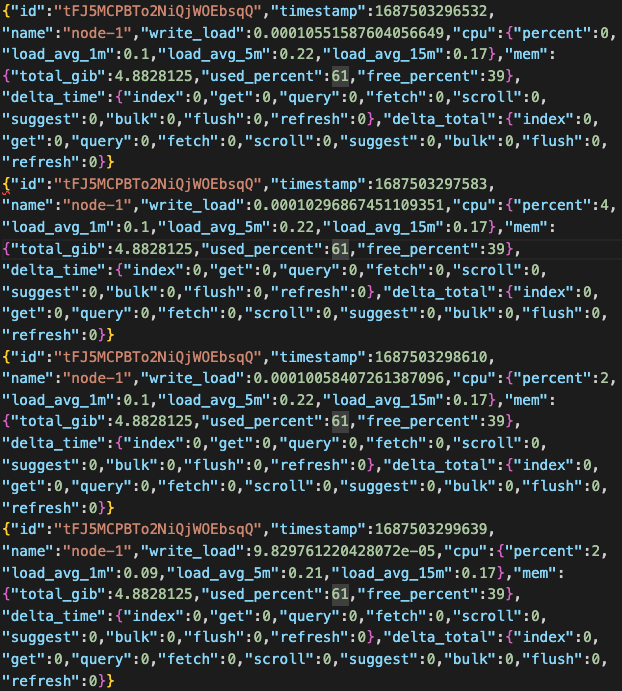
\includegraphics[width=0.8\textwidth]{chapter-4/mf-1.png}
  \caption{Hasil Pengujian Komponen \textit{Metrics Fetcher} Skenario 1}
  \label{fig:mf-1}
\end{figure}

\begin{figure}[h]
  \centering
  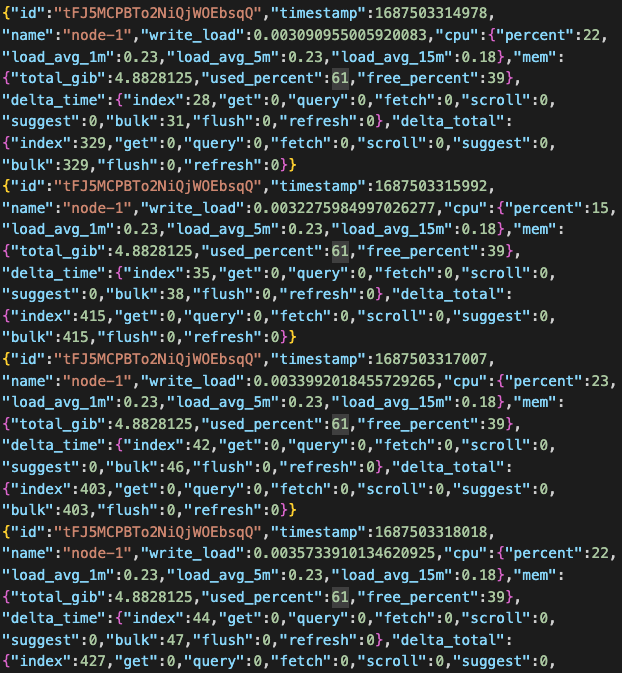
\includegraphics[width=0.8\textwidth]{chapter-4/mf-2.png}
  \caption{Hasil Pengujian Komponen \textit{Metrics Fetcher} Skenario 2}
  \label{fig:mf-2}
\end{figure}

\begin{figure}[h]
  \centering
  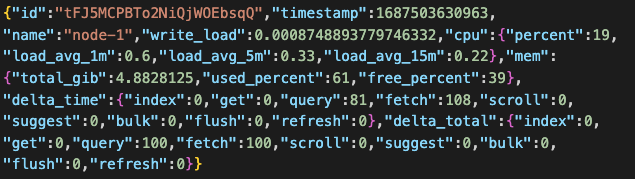
\includegraphics[width=0.8\textwidth]{chapter-4/mf-3.png}
  \caption{Hasil Pengujian Komponen \textit{Metrics Fetcher} Skenario 3}
  \label{fig:mf-3}
\end{figure}

Pengujian komponen \textbf{\textit{Metrics Fetcher}} sudah sesuai ekspektasi dan dapat dilanjutkan ke pengujian komponen lainnya.
\subsubsection{Komponen \textbf{\textit{Predictor}}}
Komponen \textbf{\textit{Predictor}} dirancangkan terdiri dari 3 buah kelas, yaitu sebagai berikut.
\begin{enumerate}
    \item \textbf{\textit{Predict Component}}
    
    Kelas ini berfungsi untuk menyimpan sebuah model ARIMA untuk sebuah variabel. Kelas ini memanfaatkan kakas pandas, statsmodels dan pmdarima untuk melakukan tanggung jawabnya.

    \item \textbf{\textit{Predict Component Factory}}
    
    Kelas ini berfungsi untuk membuat objek \textbf{\textit{Predict Component}} sebanyak variabel yang ada. 

    \item \textbf{\textit{Predict Component Storage}}
    
    Kelas ini berfungsi sebagai aggregator objek \textbf{\textit{Predict Component}} yang telah dibuat oleh \textbf{\textit{Predict Component Factory}}. Kelas ini juga berfungsi untuk meneruskan sebuah aksi kepada semua objek \textbf{\textit{Predict Component}} yang ada. Contohnya, dengan memanggil \textit{forecast} atau \textit{update data}, maka operasi akan diteruskan ke semua objek \textbf{\textit{Predict Component}}.

\end{enumerate}

\begin{figure}[h]
    \centering
    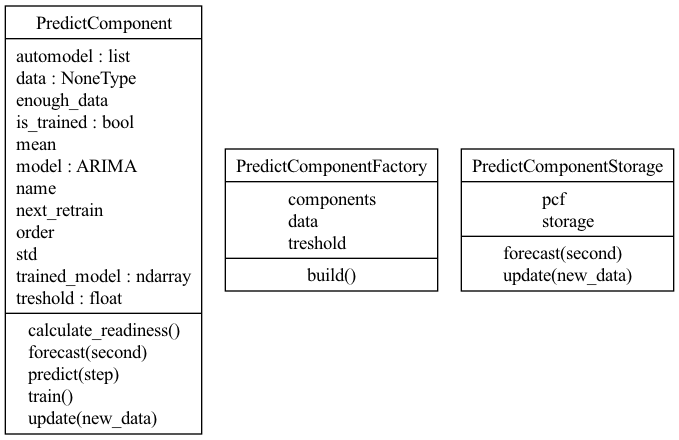
\includegraphics[width=0.8\textwidth]{chapter-4/predictor.png}
    \caption{Spesifikasi Kelas Penyusun Komponen \textit{Predictor}}
    \label{fig:predictor-spek}
\end{figure}

Secara umum, spesifikasi kelas bisa dilihat pada gambar \ref{fig:predictor-spek}. Kelas \textbf{\textit{Predict Component Storage}} akan membutuhkan \textbf{\textit{Predict Component Factory}} untuk membangun semua \textbf{\textit{Predict Component}} untuk setiap variabel yang ada. Setelah itu, terdapat operasi seperti meneruskan penambahan data serta meminta data prediksi ke setiap \textbf{\textit{Predict Component}}. Kelas ini akan digunakan oleh komponen \textbf{\textit{Flexible Control}} untuk lebih lanjutnya.
\subsubsection{Komponen \textbf{\textit{Rule Manager}}}
Komponen \textbf{\textit{Rule Manager}} dirancangkan melakukan parsing terhadap file \textit{rule} yang telah diisi oleh pengguna serta menjadi aggregator untuk melakukan pengecekan \textit{rule} yang berlangsung serta memberi informasi data prediksi kapan saja yang dibutuhkan untuk melakukan pengecekan. Parsing komponen ini menggunakan format csv dan kondisi diekspresikan dengan sintaks python. Komponen akan mengonstruksi objek \textbf{\textit{Rule}} yang akan digunakan oleh komponen \textbf{\textit{Flexible Control}}. Spesifikasi dari kedua kelas tersebut dapat dilihat pada gambar \ref{fig:rule-spek}.

\begin{figure}[h]
    \centering
    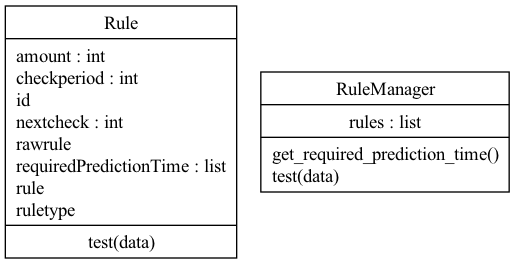
\includegraphics[width=0.8\textwidth]{chapter-4/rule.png}
    \caption{Spesifikasi Kelas Penyusun Komponen \textit{Rule Manager}}
    \label{fig:rule-spek}
\end{figure}

Sebuah \textit{rule} memiliki fungsi sebagai berikut.
\begin{enumerate}
    \item Memiliki sebuah kondisi yang akan dievaluasi dengan data prediksi pada waktu prediksi yang diinginkan. Contoh: kondisi \textit{throughput} untuk operasi X untuk 1 menit kedepan dan 5 menit kedepan lebih dari 1s, maka tingkatkan prosesor sebanyak 500m.
    \item Memiliki jumlah serta target kategori untuk diubah, dalam kasus ini pilihannya memori atau prosesor.
    \item Satuan untuk perubahan memori adalah dalam \textit{Mebibyte} atau MiB. Sedangkan untuk prosesor dalam satuan mili atau m.
    \item Sebuah \textit{rule} memiliki periode pengecekan sehingga tidak akan dicek secara terus menerus yang menyebabkan perubahan alokasi sumber daya terlalu cepat. Periode pengecekan dibuat dalam satuan sekon.
\end{enumerate}
\subsection{Komponen \textit{Resource Controller}}

Seperti yang sudah dirancangkan sebelumnya, kelas ini menggunakan \textit{Kubernetes Client API} untuk mengubah alokasi sumber daya. Diimplementasikan dengan sistem antrian, sehingga jika sejumlah rule aktif secara bersamaan, maka akan dijalankan secara berurutan. Terdapat sebuah fungsi \textit{tick} yang akan berfungsi untuk mengeksekusi antrian. Contoh simpanan file antrian dapat dilihat pada gambar \ref{fig:ex-queue-rc}. File tersebut menyimpan status alokasi sumber daya pada saat itu, kapan melakukan perubahan pada antrian berikutnya dalam waktu UNIX dan antrian yang akan dieksekusi satu per satu.

\begin{figure}[h]
    \centering
    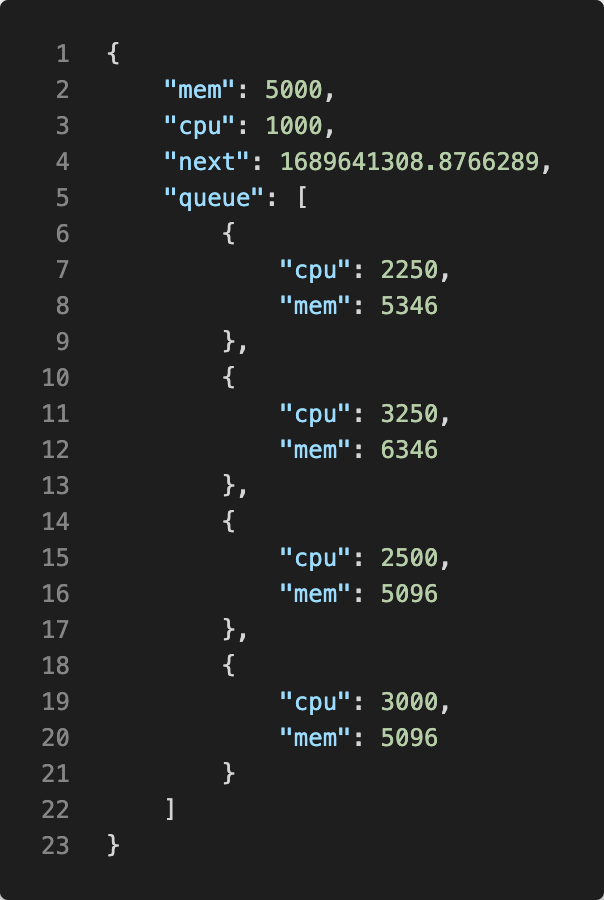
\includegraphics[width=0.45\textwidth]{chapter-4/rc-queue-ex.png}
    \caption{Contoh File Antrian Pengubahan Alokasi}
    \label{fig:ex-queue-rc}
\end{figure}

% TODO CONTOH SISTEM ANTRIAN
\subsection{Pengujian Sistem \textit{Flexible Control}}

Pada bagian ini akan dijelaskan tentang tujuan, skenario, hasil, dan analisis dari pengujian sistem sekaligus komponen \textbf{\textit{Flexible Control}}.

\subsubsection{Tujuan Pengujian}

Tujuan pengujian ini memastikan sistem \textbf{\textit{Flexible Control}} dapat berjalan dengan baik dan menghasilkan perilaku yang sesuai.

\subsubsection{Skenario Pengujian}

Pengujian terhadap komponen \textbf{\textit{Flexible Control}} dilakukan dengan beberapa skenario sebagai berikut serta ekspektasi dari pengujian yang dilakukan.
\begin{enumerate}
  \item \bfseries Sebuah \textit{rule} memenuhi kondisi untuk mengubah alokasi prosesor.\normalfont

        Prosesor akan berubah jumlahnya sesuai dengan \textit{rule} yang memenuhi kondisi. Perubahan pada spesifikasi \textit{pods} juga diekspektasikan mengikuti.

  \item \bfseries Sebuah \textit{rule} memenuhi kondisi untuk mengubah alokasi memori.\normalfont

        Prosesor akan berubah jumlahnya sesuai dengan \textit{rule} yang memenuhi kondisi. Perubahan pada spesifikasi \textit{pods} juga diekspektasikan mengikuti. Memory Used Percent akan menurun karena penambahan yang terjadi.
\end{enumerate}

\subsubsection{Hasil Pengujian dan Analisis}

Pengujian akan dilakukan dengan \textit{file rule} yang dapat dilihat pada gambar \ref{fig:ac-rule}. Terdapat dua buah \textit{rule} yang akan diuraikan sebagai berikut.

\begin{enumerate}
  \item Jika \textit{load average 1m} pada 10 detik kedepan diprediksikan diatas 0 maka akan ditambah alokasi prosesor sebesar 1000m atau sejumlah 1. Kondisi dari \textit{rule} sengaja dibuat seperti itu agar rule pasti terpenuhi.
  \item Jika \textit{memory used percent} pada 5 dan 10 detik kedepan diprediksikan diatas 60 maka akan ditambah alokasi memori sebesar 2048 mebibyte atau sejumlah 2 gibibyte (Gi). Kondisi dari \textit{rule} sengaja dibuat seperti itu agar rule pasti terpenuhi.
\end{enumerate}

Hasil dari pengujian skenario kedua dapat dilihat pada gambar \ref{fig:ac-mem}. Dan perubahan terhadap spesifikasi pods dapat dilihat pada gambar \ref{fig:ac-mem-kube}. Perubahan juga terjadi pada \textit{memory used percent} pada \textit{stream file} atau data yang ditarik oleh komponen \textbf{\textit{Metrics Fetcher}} dapat dilihat pada gambar \ref{fig:ac-mf-turun}.
Diikuti dengan hasil dari pengujian skenario pertama dapat dilihat pada gambar \ref{fig:ac-cpu}. Dapat dilihat bahwa prosesor berubah sesuai dengan ekspektasi. Perubahan pada spesifikasi \textit{pods} juga mengikuti perubahan prosesor yang dapat dilihat pada gambar \ref{fig:ac-cpu-kube}.

\begin{figure}[h]
  \centering
  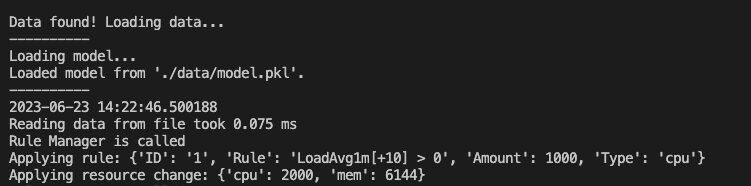
\includegraphics[width=0.8\textwidth]{chapter-4/ac-cpu.png}
  \caption{Hasil Pengujian Komponen \textit{Flexible Control} Skenario 1: Perubahan Prosesor}
  \label{fig:ac-cpu}
\end{figure}

\begin{figure}[h]
  \centering
  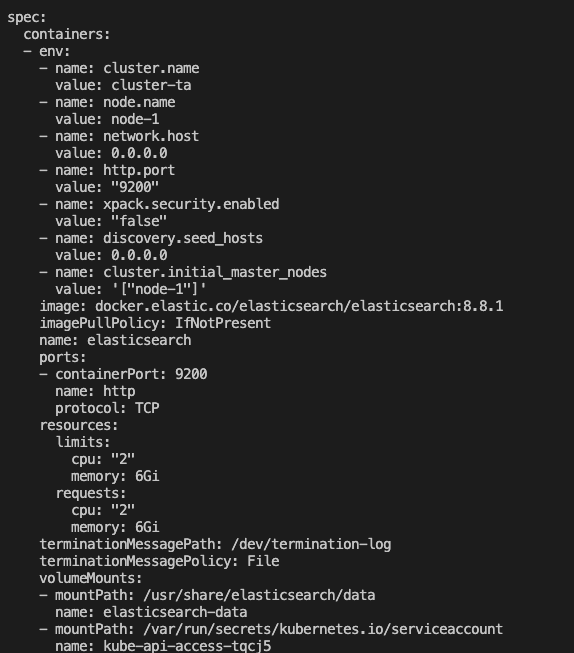
\includegraphics[width=0.8\textwidth]{chapter-4/ac-cpu-kube.png}
  \caption{Hasil Pengujian Komponen \textit{Flexible Control} Skenario 1: Perubahan Spesifikasi Kubernetes}
  \label{fig:ac-cpu-kube}
\end{figure}

\begin{figure}[h]
  \centering
  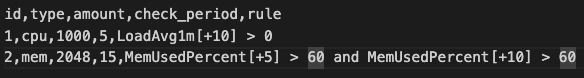
\includegraphics[width=0.8\textwidth]{chapter-4/ac-rule.png}
  \caption{File Rule untuk Pengujian Komponen \textit{Flexible Control}}
  \label{fig:ac-rule}
\end{figure}

\begin{figure}[h]
  \centering
  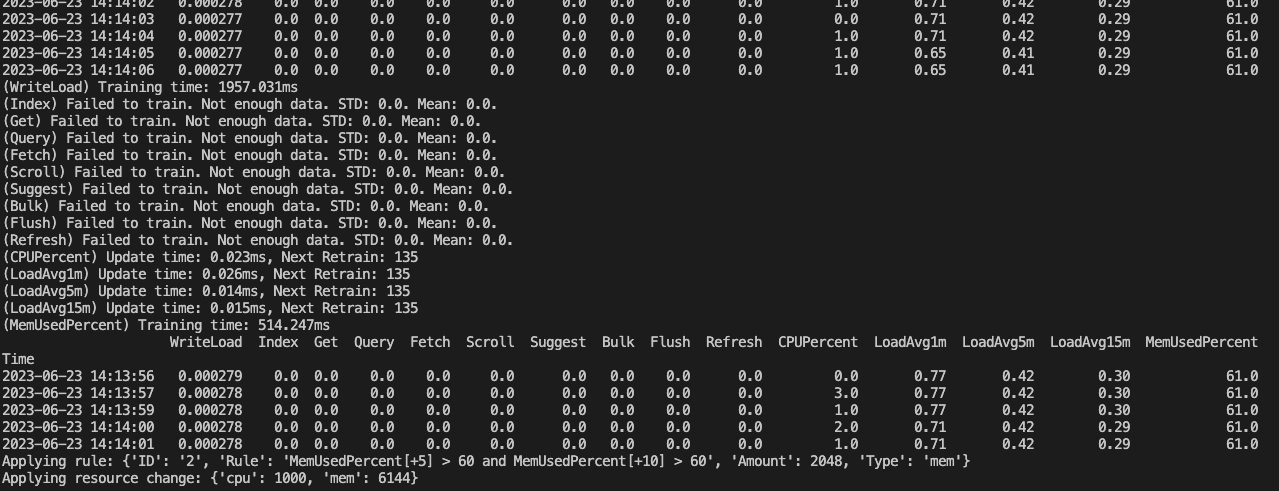
\includegraphics[width=1\textwidth]{chapter-4/ac-mem.png}
  \caption{Hasil Pengujian Komponen \textit{Flexible Control} Skenario 2: Perubahan Memori}
  \label{fig:ac-mem}
\end{figure}

\begin{figure}[h]
  \centering
  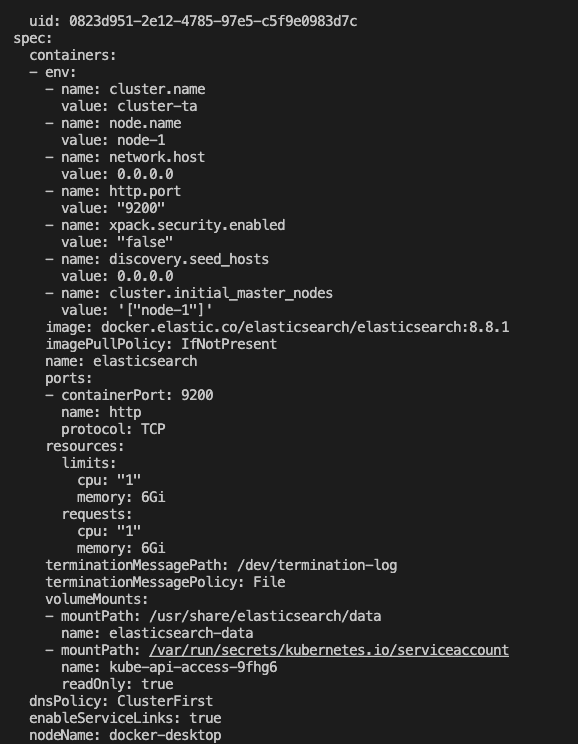
\includegraphics[width=0.8\textwidth]{chapter-4/ac-mem-kube.png}
  \caption{Hasil Pengujian Komponen \textit{Flexible Control} Skenario 2: Perubahan Spesifikasi Kubernetes}
  \label{fig:ac-mem-kube}
\end{figure}

\begin{figure}[h]
  \centering
  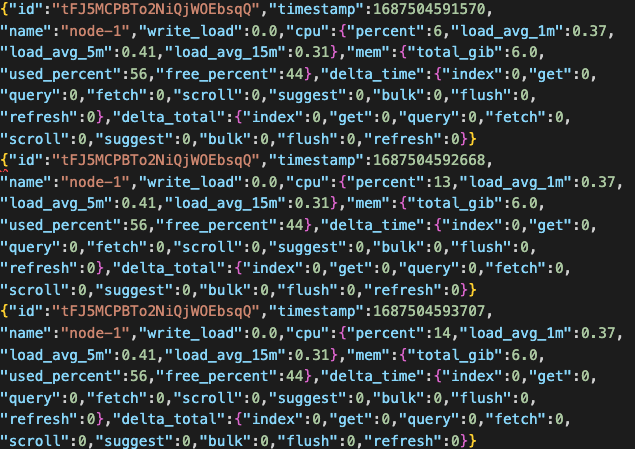
\includegraphics[width=0.8\textwidth]{chapter-4/ac-mf-turun.png}
  \caption{Hasil Pengujian Komponen \textit{Flexible Control} Skenario 2: Perubahan Memory Used Percent pada \textit{stream file}}
  \label{fig:ac-mf-turun}
\end{figure}

Pengujian komponen \textbf{\textit{Flexible Control}} sudah sesuai ekspektasi dan sistem dapat berjalan dengan baik.

\subsection{Alur Kerja Sistem}

Untuk alur kerja sistem, secara spesifik \textit{autoscaler} dengan kontrol fleksibel akan melakukan tugasnya dengan mengikuti fase-fase pada arsitektur sistem MAPE yang sudah dijelaskan pada bagian \ref{sec:arsitektur-sistem}. Pada fase-fase tersebut, ada alur kerja yang harus dilakukan oleh sistem, diantaranya sebagai berikut.

\begin{enumerate}
    \item \bfseries \textit{Monitor} \normalfont
    
        Alur pada fase ini dapat dilihat pada gambar \ref{fig:alur-monitor}.

        \begin{figure}[h]
            \centering
            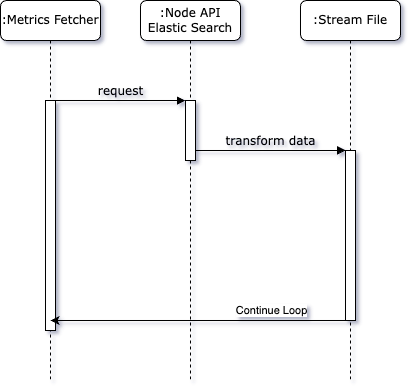
\includegraphics[width=0.7\textwidth]{chapter-3/monitor.png}
            \caption{Rancangan Alur Fase \textit{Monitor}}
            \label{fig:alur-monitor}
        \end{figure}
        
    \item \bfseries \textit{Analyse} \normalfont
    
        Fase ini memiliki alur yang dapat dilihat pada gambar \ref{fig:alur-analysis}.

        \begin{figure}[h]
            \centering
            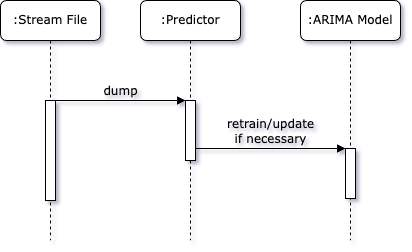
\includegraphics[width=0.8\textwidth]{chapter-3/analysis.png}
            \caption{Rancangan Alur Fase \textit{Analysis}}
            \label{fig:alur-analysis}
        \end{figure}
        
    \item \bfseries \textit{Planning} \normalfont
    
        Dalam melakukan fase ini, alur yang akan dilalui oleh sistem dapat dilihat pada gambar \ref{fig:alur-planning}.

        \begin{figure}[h]
            \centering
            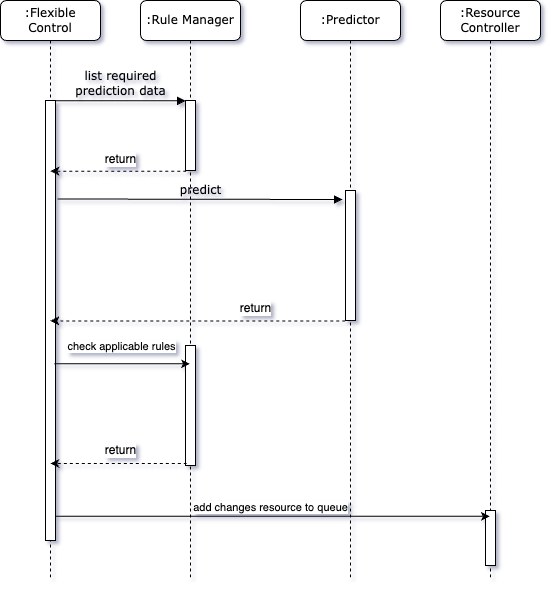
\includegraphics[width=0.5\textwidth]{chapter-3/planning.png}
            \caption{Rancangan Alur Fase \textit{Planning}}
            \label{fig:alur-planning}
        \end{figure}

    \item \bfseries \textit{Execution} \normalfont
    
        Apabila terdapat hal yang perlu dieksekusi, fase ini akan memiliki alur yang dapat dilihat pada gambar \ref{fig:alur-execution}. Apabila tidak ada yang perlu dieksekusi, sistem akan melanjutkan ke loop berikutnya dan melewati alur pada fase ini.

        \begin{figure}[h]
            \centering
            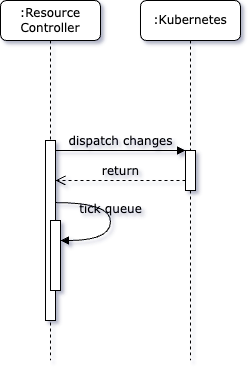
\includegraphics[width=0.35\textwidth]{chapter-3/execution.png}
            \caption{Rancangan Alur Fase \textit{Execution}}
            \label{fig:alur-execution}
        \end{figure}
\end{enumerate}

\subsection{Hubungan Kubernetes, \textit{Elastic Search} dengan \textit{Autoscaler} dengan Sistem Kontrol Fleksibel}

Pada bagian ini, keterhubungan antara 3 buah sistem yang berbeda akan dijelaskan melalui gambar \ref{fig:rancangan-sistem}. Kubernetes akan mengekspos API yang akan dipakai oleh \textit{Autoscaler} dengan Sistem Kontrol Fleksibel melalui \textit{Kubernetes Client Library}. Sedangkan, \textit{Elastic Search} akan mengekspos API yang berbentuk REST API yang akan dipakai oleh \textit{Autoscaler} dengan Sistem Kontrol Fleksibel melalui \textit{HTTP Client}.

\begin{figure}[h]
    \centering
    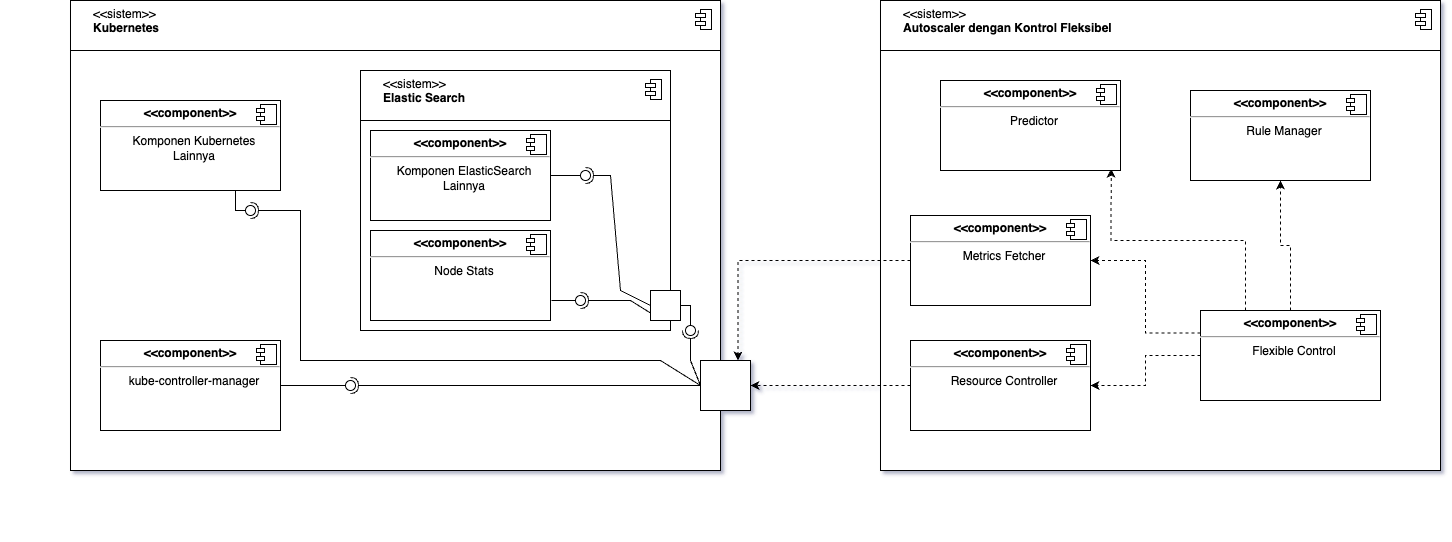
\includegraphics[width=1.1\textwidth]{chapter-3/component.png}
    \caption{Rancangan Sistem}
    \label{fig:rancangan-sistem}
\end{figure}